% Revised scientific proposal, 14 November 2026. ACL 2015 course template.
% Compile in the same Overleaf project as the original, with acl2015.sty.
\documentclass[11pt]{article}
\usepackage{acl2015}
\usepackage{times}
\usepackage{url}
\usepackage{latexsym}
\usepackage{booktabs,tabularx,array}
\usepackage{tikz}
\usetikzlibrary{arrows.meta,positioning}
\usepackage[T1]{fontenc}
\usepackage[utf8]{inputenc}
\usepackage{amsmath}
\usepackage{enumitem}
\emergencystretch=2em
\title{Clickbait Without the Click:\\Linguistic Cues under Temporal Shift\\Project Proposal for NLP, Winter 2026/27}
\author{Igor Ko{\l}odziej, Hubert Kowalski, Adam Kaniasty, Mateusz Iwaniuk \\
Warsaw University of Technology\\Supervisor: Anna Wr{\'o}blewska\\{\footnotesize Template: Anna Wr{\'o}blewska (Warsaw University of Technology), adapted from the ACL 2015 formatting template.}}
\date{}
\newcommand{\mF}{macro-$F_1$}
\newcommand{\cue}[1]{\textsf{#1}}
\begin{document}
\maketitle
\begin{abstract}
We test whether a \emph{prespecified, interpretable} set of twelve text-only cues improves clickbait detection beyond fixed sentence embeddings when the test period changes. Our primary experiment isolates the cue contribution: the same all-MiniLM-L6-v2 embeddings, logistic-regression family, data partitions and tuning protocol are used with and without the twelve cues. Unlike a random-only hybrid-model comparison, we quantify cue gains across three chronological windows, their random-versus-temporal gap, feature-family failures and uncertainty. We audit duplicate and article overlap to strengthen the validity of chronological comparisons. The publicly released Webis-Clickbait-17 training corpus is primary, Webis-Clickbait-16 supplies an external evaluation, and a separate teaser--article context analysis tests additional information mechanisms. A recent YouTube corpus and an open decision model offer additional evaluations if resources permit. Our contribution is an auditable test of \emph{when and why} linguistic cues help, and the mechanisms behind their successes and failures.
\end{abstract}

\section{Research questions and contribution}
The prediction input is a \emph{social-media teaser} (\texttt{postText}); the target is the corpus's official binary \texttt{truthClass}, not observed clicks, misinformation or reader satisfaction. We ask whether shallow linguistic mechanisms add information not captured by frozen embeddings \emph{under chronological evaluation}, rather than merely improve a random test.
\paragraph{H1: controlled cue value.} Adding the twelve prespecified cues to identical frozen embeddings increases out-of-time \mF{} (C minus B) on the untouched April 2017 test. The paired difference and its uncertainty provide the primary test of this hypothesis.
\paragraph{H2: robustness rather than random-split gains.} Cues retain a beneficial C--B effect across the February, March and April held-out tests; an apparent gain restricted to random splits does \emph{not} support temporal robustness. We compare the resulting effect sizes with grouped-random evaluation.
\paragraph{H3: mechanisms, not just a score.} The contribution of referential withholding, engagement, emotional framing and specificity differs across months; leave-one-family-out ablations and stratified errors will reveal where apparent improvements fail. We quantify each family's contribution through controlled ablations.

\paragraph{H4: context information gain (secondary).} On identical article-complete instances, inexpensive teaser--article relation cues improve temporal macro-$F_1$ beyond a context-aware classifier with the twelve teaser cues. This comparison measures the incremental value of relational information.

\textbf{Independent contribution.} The study contributes (i) a reproducible, mechanism-driven specification of twelve interpretable cues; (ii) a controlled test of their incremental value over fixed sentence representations; (iii) a comparison of chronological and article-grouped random evaluation, including uncertainty, feature-family stability and systematic error analysis; (iv) a matched-input teaser--article consistency experiment; and (v) a reusable cross-partition overlap audit. Together, these experiments examine both the predictive value and the conditions under which lightweight linguistic signals remain useful. Our design extends the informativeness-based hybrid approach of Michaluk et al.\ \cite{michaluk2026} in several complementary directions: we isolate the effect of handcrafted cues while keeping embeddings and classifier fixed, evaluate their stability across chronological windows rather than relying only on a mixed-source random split, and examine whether teaser--article relationships add information beyond teaser-level cues. This enables a mechanism-oriented analysis of generalization, rather than a comparison based solely on aggregate classification scores.

\section{Related work and verifiable comparisons}
Feature-based work by Potthast et al.\ \cite{potthast2016} established clickbait cues in publisher tweets, while Biyani et al.\ \cite{biyani2016} showed that article informality and metadata can be useful in a different news-stream dataset. Chakraborty et al.\ \cite{chakraborty2016} introduced a large headline resource subsequently reused by many studies; its random-split results should not be transferred to our Webis setting. Anand et al.\ \cite{anand2017} showed strong sequence-based headline classification, while Wei and Wan \cite{wei2017} separated ambiguous from misleading Chinese headlines. Potthast et al.\ \cite{potthast2018} established the five-annotator Webis-17 labels and their disagreement; the Clickbait Challenge overview \cite{potthast2018challenge} describes benchmark evaluation, but the self-attentive winning entry is Zhou \cite{zhou2017}.

Indurthi et al.\ \cite{indurthi2020} predict clickbait \emph{strength} on Webis; Yi et al.\ \cite{yi2022} combine text and labels in contrastive modelling. Brosco\c{t}eanu and Ionescu \cite{roclico2023} test publisher-disjoint Romanian articles, closest to source separation, whereas Wu et al.\ \cite{wu2020} compare title style with title--body interaction on news and clickbait benchmarks. Andjeli\'c et al.\ \cite{andelic2025} provide a Croatian-language test of transfer across linguistic contexts. Reimers and Gurevych \cite{reimers2019sbert} motivate fixed sentence embeddings; Wang et al.\ \cite{wang2020minilm} motivate compact encoders, without providing a clickbait result. Guo et al.\ \cite{guo2017calibration} and Desai and Durrett \cite{desai2020} motivate calibration diagnostics. Crucially, S\o gaard et al.\ \cite{sogaard2021} challenge overly optimistic random splitting, and R\"ottger and Pierrehumbert \cite{rottger2021} show why social-language changes do not automatically translate into downstream temporal degradation. Recent efficient clickbait classification \cite{kuntur2026} provides an additional low-cost reference, without establishing our controlled test.

\begin{table*}[t]
\centering
\caption{Selected published evidence (not a league table). \emph{Test} denotes the authors' evaluation partition; \emph{CV} denotes cross-validation. `---' denotes a methodological study with no comparable clickbait score. Averaging is stated for each quoted $F_1$ value. Non-clickbait tasks and unlike input modalities are identified.}
\label{tab:sota}
\setlength{\tabcolsep}{3pt}\renewcommand{\arraystretch}{1.04}\scriptsize
\begin{tabularx}{\textwidth}{@{}p{2.10cm}p{3.10cm}X p{2.25cm}@{}}
\toprule
Work & Method and input & Dataset / evaluation partition & Published value (type)\\
\midrule
Potthast et al. 2016 & RF, tweet cues & Webis-16 (2,992); random 2:1, test & ROC-AUC .79\\
Biyani et al. 2016 & Boosted trees; title/body/URL & Yahoo news; 3,000 train, 1,073 test & $F_1$ .749 (weighted); .603 (positive)\\
Anand et al. 2017 & BiLSTM; headline & Balanced headlines (15k); ten-fold CV & $F_1$ .9819 (averaging not specified; non-comparable)\\
Wei and Wan 2017 & SVM/rules, co-training; Chinese & Ambiguity 2,924; misleadingness 2,608; random 3:1 test & $F_1$ .753/.724 (averaging not specified)\\
Potthast et al. 2018 & Five-annotator corpus & Webis-17 (38,517); annotation, no classifier split & Fleiss $\kappa$ .21/.36 (four-/two-level)\\
Zhou 2017 & Self-attentive BiGRU; posts & Clickbait Challenge 2017 official held-out test (18,979) & MSE .033; $F_1$ .683 (challenge truthClass)\\
Indurthi et al. 2020 & RoBERTa, boosted regression; post & Clickbait Challenge 2017 official test & MSE .0242; $F_1$ .7408 (challenge truthClass)\\
Yi et al. 2022 & Contrastive variational model; post/article & Webis-derived 17,588/2,000/17,554 train/dev/test & $F_1$ .694 (macro, test)\\
Brosco\c{t}eanu et al. 2023 & Contrastive Ro-BERT; article & RoCliCo 6,806 train; 1,507 publisher-disjoint test & $F_1$ .9199 (macro, test)\\
Wu et al. 2020 & Style-aware attention with title/body & Clickbait Challenge; 2,495 released development items used as test (Table 1) & $F_1$ .733 (positive-class; test)\\
Andjeli\'c et al. 2025 & BERTi\'c; Croatian headlines & CLIC 2,907; 80/10/10, test & $F_1$ .776 (averaging not specified)\\
Michaluk et al. 2026 & Embeddings + cues + XGBoost; titles & Mixed sources; balanced 40k; random 80/10/10, test & $F_1$ .864--.909 (paper's ablation; averaging not specified)\\
Reimers and Gurevych 2019 & Sentence-BERT; transfer & SentEval tasks; ten-fold CV, not clickbait & Mean accuracy 87.41\%\\
Wang et al. 2020 & MiniLM; transfer & SQuAD2 / SST-2, development; not clickbait & $F_1$ 72.4 (SQuAD2); accuracy 91.0\%\\
Guo et al. 2017 & Temperature scaling; TreeLSTM & SST-binary; held-out test; not clickbait & ECE 6.63\% to 1.84\%\\
S\o gaard et al. 2021 & Split-design study; NLP & Multiple NLP tests; split-protocol analysis & --- (methodological)\\
R\"ottger et al. 2021 & Temporal BERT adaptation & Social-media classification across years & --- (temporal analysis)\\
Desai and Durrett 2020 & Transformer calibration & Three NLP tasks; in/out of domain & --- (calibration analysis)\\
\bottomrule
\end{tabularx}
\end{table*}

\section{Datasets and provenance}
\textbf{Webis-Clickbait-17 --- READY.} The openly accessible labelled training archive \texttt{clickbait17-train-170630.zip} (Zenodo, CC BY 4.0) contains 19,538 posts (4,761 positive; 24.37\%) with identifiers, December 2016--April 2017 timestamps and differently ordered \texttt{instances.jsonl}/\texttt{truth.jsonl}, joined by ID. The archive does \emph{not} provide publisher IDs or original target URLs. The official additional test release (18,979 posts) is \textbf{RESTRICTED}: its labels are exposed only through TIRA, so it is not used in our experiments \cite{potthast2018,potthast2018challenge}. Five annotators score 0, .33, .66 or 1; our classification label is the \emph{released} \texttt{truthClass}, defined from the modal five-person rating: 0 or .33 maps to non-clickbait, .66 or 1 to clickbait; when ratings have multiple modes, the fifth judgment breaks the tie (as specified in the official corpus paper), rather than imposing a new \texttt{truthMean} threshold. We preserve \texttt{truthJudgments} and \texttt{truthMean} only for disagreement/error analysis; no alternate labels are inferred.

The first audit removed 54 empty teasers and 411 duplicate occurrences, leaving 19,073 posts (4,529 positives). A subsequent \emph{local pilot export}, after article-key filtering, reports 18,682 posts (4,448 positive, 23.81\%); its 391-row difference from the earlier stage is \emph{not yet reconciled}. We treat 18,682 as \emph{pilot analysis size}, and the pipeline records row-level exclusions and final sample identifiers after the discrepancy and leakage audit. Monthly provisional counts are in Table~\ref{tab:months}.

\begin{table}[t]
\centering\small\setlength{\tabcolsep}{5pt}
\caption{Local pilot, post-filter Webis-17; post-filter counts from the current pilot run.}
\label{tab:months}
\begin{tabular}{@{}lrrr@{}}\toprule
Month & All & Clickbait & Positive \%\\\midrule
Dec 2016 & 3,832 & 1,012 & 26.4\\
Jan 2017 & 3,848 & 884 & 23.0\\
Feb 2017 & 3,504 & 814 & 23.2\\
Mar 2017 & 3,918 & 908 & 23.2\\
Apr 2017 & 3,580 & 830 & 23.2\\\midrule
Total & 18,682 & 4,448 & 23.8\\\bottomrule
\end{tabular}
\end{table}

\textbf{Webis-Clickbait-16 --- READY (publicly available); external evaluation.} The Webis record \url{https://zenodo.org/records/3251557} (v1; DOI 10.5281/zenodo.3251557) offers \texttt{corpus-webis-clickbait-16.zip} under CC BY 4.0: 2,992 English tweets from 20 publishers, 767 positive (25.6\%), based on majority votes of three annotators \cite{potthast2016}. Its English tweet text and majority-vote labels form the external test input, with cross-corpus overlap and label correspondence checked during preprocessing.

\textbf{Optional cross-domain extension: YTClickbait21K.} Islam et al.\ \cite{islam2026} release 21,238 English YouTube videos (9,653 positive; 11,585 negative), title/description, upload dates and three-annotator labels, via Figshare \url{https://doi.org/10.6084/m9.figshare.31891576} (CC BY 4.0; \texttt{main\_dataset.csv}). If time permits, evaluate \emph{titles only} with unchanged Webis-trained models after checking video dates and overlap. YouTube versus news-post data and multimodal annotation mean changes cannot be attributed to time alone; thumbnails, video metadata and channels are \emph{not} inputs.

\section{Models and twelve operational cues}
The primary A/B/C comparison uses the same cleaned \texttt{postText} only; article content, images and publisher metadata are excluded from this main prediction input. A \emph{secondary, separately labelled context experiment} uses teaser text, linked \texttt{targetTitle} and a fixed-length excerpt of available \texttt{targetParagraphs} for \emph{all} participating systems, with matched records and identical train/validation/test partitions. Thus article context is never provided exclusively to the proposed classifier. The context experiment tests whether interpretable \emph{relations} across teaser and article add information, while the primary twelve-cue test remains deployable when only teasers exist.

\textbf{A: lexical baseline.} Word 1--2-gram and character 3--5-gram term-frequency/inverse-document-frequency (TF--IDF) vectors followed by L2-regularized logistic regression (LR). \textbf{B: embedding baseline.} Fixed \texttt{all-MiniLM-L6-v2} sentence representations (384 dimensions), cached and followed by LR. \textbf{C: controlled hybrid.} Exactly B's cached vectors concatenated with \emph{twelve} hand-defined scalar cues and the same LR family. The operational definitions, patterns and denominators are in Appendix~\ref{app:cues}; no test labels enter cue selection. Scalers, vocabulary and all fitted transforms are learned on training data only. All models use \texttt{class\_weight=balanced}; A, B and C select regularization from the \emph{same fixed grid} by validation \mF{}. This is a matched model-class and tuning-budget comparison, not a claim to reproduce the seed paper's XGBoost configuration.

\begin{figure}[t]
\centering
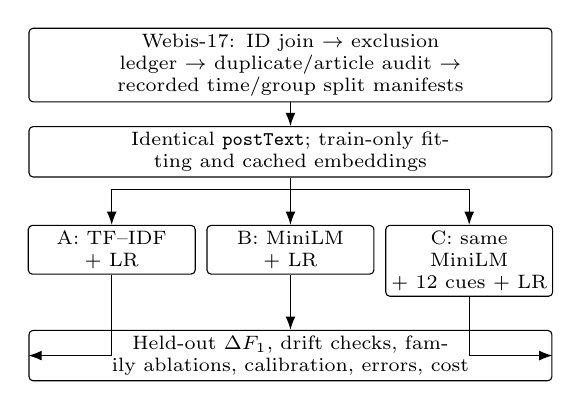
\begin{tikzpicture}[>=Latex,node distance=3mm,
 block/.style={draw,rounded corners=1.5pt,align=center,inner sep=2pt,font=\scriptsize,text width=6.5cm},
 narrow/.style={draw,rounded corners=1.5pt,align=center,inner sep=2pt,font=\scriptsize,text width=1.98cm}]
\node[block] (d) {Webis-17: ID join $\rightarrow$ exclusion ledger $\rightarrow$ duplicate/article audit $\rightarrow$ recorded time/group split manifests};
\node[block,below=of d] (p) {Identical \texttt{postText}; train-only fitting and cached embeddings};
\node[narrow,below=6mm of p,xshift=-2.27cm] (a) {A: TF--IDF\\+ LR};
\node[narrow,below=6mm of p] (b) {B: MiniLM\\+ LR};
\node[narrow,below=6mm of p,xshift=2.27cm] (c) {C: same MiniLM\\+ 12 cues + LR};
\node[block,below=7mm of b] (e) {Held-out $\Delta F_1$, drift checks, family ablations, calibration, errors, cost};
\draw[->] (d)--(p);
\draw[->] (p.south)--++(0,-1.5mm)-|(a.north);
\draw[->] (p.south)--(b.north);
\draw[->] (p.south)--++(0,-1.5mm)-|(c.north);
\draw[->] (a.south)|-(e.west);
\draw[->] (b.south)--(e.north);
\draw[->] (c.south)|-(e.east);
\end{tikzpicture}
\caption{Primary three-system evaluation; optional external and decision-model checks reuse the defined test instances.}
\label{fig:pipeline}
\end{figure}

\paragraph{Mechanism-oriented cues.} Instead of generic length and capitalization alone, we operationalize four \emph{interpretive} families: referential withholding (features 1--3), reader engagement (4--6), affect/uncertainty (7--9), and headline specificity/packaging (10--12). Ratios use token or character denominators so a long post is not automatically assigned stronger clickbait scores. Several mechanisms overlap previous lexical work; the novelty claimed is the prespecified \emph{combination, controls and robustness analysis}, not ownership of isolated patterns.

\paragraph{Matched teaser--article consistency experiment (secondary).} On Webis-17 examples with usable \texttt{targetTitle} and \texttt{targetParagraphs}, we also compare $A_{\mathrm{ctx}}$ (TF--IDF on the same serialized teaser/title/body excerpt), $B_{\mathrm{ctx}}$ (MiniLM on that serialization plus LR), $C_{\mathrm{ctx}}$ ($B_{\mathrm{ctx}}$ plus the twelve teaser cues), and $D_{\mathrm{ctx}}$ ($C_{\mathrm{ctx}}$ plus three transparent relation cues). The latter are (R1) normalized content-word overlap of teaser versus article lead; (R2) fraction of teaser named entities absent from the lead (spaCy entities, explicit empty-set rule); and (R3) MiniLM cosine similarity between teaser and lead, with the same cached encoder and no label-informed training. The incremental \emph{D--C} difference isolates relation features, while the \emph{B--C} difference isolates the original twelve cues under identical context. The same complete-case rows are used in all four systems and compared against the teaser-only models on those very rows. The lead is the first 96 word tokens from non-empty \texttt{targetParagraphs}, not the full linked article. This context-based study is not used as the basis of Webis-16 or YouTube results and makes no claims when article fields are missing. The three relation cues are \emph{additional to}, not substituted into, the twelve teaser cues. Prior title--body interaction work \cite{wu2020} motivates the design; its novelty here is the matched, low-cost, time-held-out intervention rather than the idea of title--body comparison itself.

\paragraph{Open decision-model comparison (optional).} If compute permits, Jeff-Qwen3.5 (\url{https://github.com/firelex/jeff}) supplies a genuinely different decision-model family. We compare (i) zero-shot binary classification, (ii) few-shot with a fixed, balanced demonstration set selected only from each window's training period, and (iii) a low-rank adaptation (LoRA) trained on that window's training partition. Each option uses the same post text and fixed label descriptions; the Jeff revision, prompt wording, demonstration selection, option order and class-probability extraction are recorded. Jeff's native score/choice interface is used rather than assuming that it generates free-form labels. Any adapted comparison across all windows requires a separate adapter for each window; a main-window-only LoRA result is explicitly labelled as such. These experiments compare method families rather than validate the causal role of our twelve cues. Architectural Jeff--cue fusion is not part of the planned experiments.

\section{Evaluation and validation protocol}
\textbf{Chronology (primary).} Three expanding-origin windows have the following train/validation/test months and provisional counts: (W1) Dec/Jan/Feb: 3,832/3,848/3,504; (W2) Dec--Jan/Feb/Mar: 7,680/3,504/3,918; (W3, main) Dec--Feb/Mar/Apr: 11,184/3,918/3,580. Validation never follows test. We require $N_{\mathrm{test}}\geq1{,}000$; if a cleaned month falls below this threshold, its window is excluded with a documented explanation rather than merged into an unseen future period. All three pilot windows exceed this threshold; preprocessing may change final counts.

\textbf{Random diagnostic.} Three seeded, article-grouped, label-stratified random splits use \texttt{article\_group\_key}: normalized \texttt{targetTitle}, falling back to record ID if unavailable. Groups, not individual rows, are assigned to partitions; with one row per title after filtering, group and row counts can be nearly identical. The \emph{same split proportions} as the main chronological split are used where possible. Group strata use a prespecified group-level majority label, with ties resolved consistently, and the algorithm records any post-level deviation from target balance. Random results diagnose protocol optimism, not a second claim about future time.

\textbf{Leakage-control audit.} A reusable checker (i) hashes normalized \texttt{postText}, titles and available stable IDs, (ii) proposes approximate duplicates using character n-gram similarity/MinHash, (iii) reviews a fixed sample near the threshold, and (iv) reports exact and near matches \emph{across} each train/validation/test boundary and between Webis-16 and Webis-17. Article groups are never split in a random protocol. For chronological windows, any linked repeated article or identified high-confidence duplicate crossing a boundary is assigned to the earliest eligible partition and later occurrences excluded; we record exclusions by reason. Audit thresholds are specified from the development data and applied consistently across test partitions. Publisher identity cannot be preserved when IDs are absent; we do not infer source-generalization claims from missing identifiers.

\textbf{Data pilot and shift tests.} Exploratory data analysis (EDA) reconciles 19,073 versus 18,682 retained rows and show monthly positivity, feature distributions, duplicate rates, and length/topic proxies. We quantify changes in feature distributions and class prevalence across months, using bootstrap intervals to characterize their variability. We relate changes in cue effectiveness to month-level feature distributions and class prevalence, reporting uncertainty for each chronological comparison.

\textbf{Metrics and inference.} The prespecified primary comparison is \(\Delta_t=F_{1,\mathrm{macro}}(C,t)-F_{1,\mathrm{macro}}(B,t)\). We report all three $\Delta_t$, the April paired bootstrap 95\% confidence interval (resampling test instances/clusters, no test-time tuning), and the difference between grouped-random and temporal outcomes. Secondary metrics are positive-class precision, recall and $F_1$, average precision (with each test prevalence), Brier score, reliability diagrams, confusion matrices, runtime and peak memory. No cross-month calibration comparison is interpreted without accounting for class prevalence. April serves as the final held-out test; all tuning uses the March validation partition. Family leave-one-out ablations (four families), a matched-row context experiment, per-cue distribution/stability plots, and at least 20 misclassified or model-disagreement examples grouped by named error categories will include low- versus high-annotator-agreement cases. We log hardware, package versions, seeds, transformations, training times and retrieval dates.

\section{Deliverables and responsibility}
Three deliverables are (D1) a documented, deduplicated ID-joined loader, exclusion ledger, overlap audit and immutable split manifests; (D2) reproducible A/B/C experiments with twelve defined cues, three chronological windows, three grouped-random diagnostics, family ablations and the matched-context experiment; (D3) statistical uncertainty, feature/error/calibration/compute analyses, scientific report and presentation. External Webis-16 is a diagnostic if text/labels are compatible; YTClickbait21K and Jeff are \emph{optional}, and do not determine the core project's completion.

\begin{table}[t]
\centering\scriptsize\setlength{\tabcolsep}{3pt}
\caption{Accountability: one primary owner per deliverable, named reviewer.}\label{tab:roles}
\begin{tabularx}{\columnwidth}{@{}p{1.35cm}p{1.16cm}X@{}}\toprule
Owner & Reviewer & Concrete deliverable\\\midrule
Adam & Igor & Join/clean scripts; provenance and Webis-16 audit\\
Hubert & Adam & TF--IDF, 12-cue extractor, family ablations\\
Igor & Mateusz & MiniLM cache; B/C models and training protocol\\
Mateusz & Hubert & Split checks, uncertainty, calibration and 20 errors\\\bottomrule
\end{tabularx}
\end{table}


\begin{table}[t]
\centering\scriptsize\setlength{\tabcolsep}{3pt}
\caption{Updated weekly milestones. Dates are planning targets, not claimed completed results.}\label{tab:weekly}
\begin{tabularx}{\columnwidth}{@{}p{1.5cm}X p{1.10cm}@{}}\toprule
Period & Concrete output & Owner\\\midrule
4--18 Nov & Phase-1 source/feedback audit; PoC + first cue specification & Igor\\
19--25 Nov & Monthly EDA, 391-row reconciliation and article audit & Adam\\
26 Nov--2 Dec & Fixed 12-cue extraction; three-way proof of concept & Hubert\\
3--9 Dec & Duplicate-check thresholds, final split manifests & Adam\\
10--16 Dec & B/C matched temporal and grouped-random runs & Igor\\
17--23 Dec & Family ablations, calibration, 20 categorized errors & Mateusz\\
24--30 Dec & Contingency; optional external text compatibility & Adam\\
31 Dec--6 Jan & Independent reproduction and report checks & Hubert\\
7--13 Jan & Final paper, source, video and question session & Igor\\\bottomrule
\end{tabularx}
\end{table}

\section{Ethics, limitations and record keeping}
\textbf{Data and licensing.} Webis-17 and Webis-16 records are distributed under CC BY 4.0 (attribution retained); the optional Figshare corpus is CC BY 4.0. Public posts can contain names, handles and links. We do not enrich user profiles, scrape new personal information or release full text in split manifests: the manifests will contain IDs, partition assignment, group keys and checksum/provenance only. Access dates, source links, excluded counts and corpus terms will be logged. We cannot recover publisher-disjoint $F_1$ without reliable publisher IDs.

\textbf{Limits.} Small chronological distance, temporal-topic confounding, pretrained embedding exposure, uncertain text availability across corpora, semantic similarity false positives, and differing label definitions constrain interpretation. Article consistency is evaluated separately from the primary teaser-only comparison and cannot be assumed to generalize to text-only external corpora. Optional YouTube labels were influenced by multimodal review and therefore cannot isolate time shift.

\textbf{AI assistance and contributions.} AI assistants (GPT 6.1 by OpenAI and Perplexity) were used for literature discovery, initial synthesis of prior work, and language verification/copyediting of the final document draft. 

\begin{thebibliography}{99}\small
\bibitem[Potthast et al., 2016]{potthast2016} M. Potthast, S. K\"opsel, B. Stein, and M. Hagen. 2016. Clickbait detection. \emph{ECIR}, 810--817. \url{https://doi.org/10.1007/978-3-319-30671-1_72}.
\bibitem[Biyani et al., 2016]{biyani2016} P. Biyani, K. Tsioutsiouliklis, and J. Blackmer. 2016. ``8 amazing secrets for getting more clicks'': Detecting clickbaits in news streams using article informality. \emph{AAAI}, 94--100. \url{https://ojs.aaai.org/index.php/AAAI/article/view/10388}.
\bibitem[Chakraborty et al., 2016]{chakraborty2016} A. Chakraborty, B. Paranjape, S. Kakarla, and N. Ganguly. 2016. Stop Clickbait: Detecting and preventing clickbaits in online news media. \emph{ASONAM}, 9--16. \url{https://doi.org/10.1109/ASONAM.2016.7752207}.
\bibitem[Anand et al., 2017]{anand2017} A. Anand, T. Chakraborty, and N. Park. 2017. We used neural networks to detect clickbaits: You won't believe what happened next! \emph{ECIR}, 541--547.
\bibitem[Wei and Wan, 2017]{wei2017} W. Wei and X. Wan. 2017. Learning to identify ambiguous and misleading news headlines. \emph{IJCAI}, 4172--4178. \url{https://www.ijcai.org/proceedings/2017/0582.pdf}.
\bibitem[Potthast et al., 2018]{potthast2018} M. Potthast et al. 2018. Crowdsourcing a large corpus of clickbait on Twitter. \emph{COLING}, 1498--1507. \url{https://aclanthology.org/C18-1127/}.
\bibitem[Potthast et al., 2018b]{potthast2018challenge} M. Potthast et al. 2018. The Clickbait Challenge 2017: Towards a regression model for clickbait strength. \emph{arXiv:1812.10847}. \url{https://arxiv.org/abs/1812.10847}.
\bibitem[Zhou, 2017]{zhou2017} Y. Zhou. 2017. Clickbait detection in tweets using self-attentive network. \emph{arXiv:1710.05364}. \url{https://arxiv.org/abs/1710.05364}.
\bibitem[Indurthi et al., 2020]{indurthi2020} V. Indurthi, B. Syed, M. Gupta, and V. Varma. 2020. Predicting clickbait strength in online social media. \emph{COLING}, 4835--4846. \url{https://aclanthology.org/2020.coling-main.425/}.
\bibitem[Yi et al., 2022]{yi2022} X. Yi et al. 2022. Clickbait detection via contrastive variational modelling of text and label. \emph{IJCAI}, 4475--4481.
\bibitem[Brosco\c{t}eanu and Ionescu, 2023]{roclico2023} D.-M. Brosco\c{t}eanu and R. T. Ionescu. 2023. A novel contrastive learning method for clickbait detection on RoCliCo. \emph{Findings of EMNLP}, 9547--9555.
\bibitem[Wu et al., 2020]{wu2020} C. Wu, F. Wu, T. Qi, and Y. Huang. 2020. Clickbait detection with style-aware title modeling and co-attention. \emph{CCL 2020}, 1143--1154. \url{https://aclanthology.org/2020.ccl-1.106/}.
\bibitem[An\dj eli\'c et al., 2025]{andelic2025} M. An\dj eli\'c et al. 2025. What makes you CLIC: Detection of Croatian clickbait headlines. \emph{Slavic NLP}, 116--123.
\bibitem[Michaluk et al., 2026]{michaluk2026} W. Michaluk, T. Urban, M. Kubita, S. Kuntur, and A. Wr\'oblewska. 2026. Click it or leave it: Detecting and spoiling clickbait with informativeness measures and large language models. \emph{arXiv:2602.18171}. \url{https://arxiv.org/abs/2602.18171}.
\bibitem[Reimers and Gurevych, 2019]{reimers2019sbert} N. Reimers and I. Gurevych. 2019. Sentence-BERT. \emph{EMNLP-IJCNLP}, 3982--3992. \url{https://doi.org/10.18653/v1/D19-1410}.
\bibitem[Wang et al., 2020]{wang2020minilm} W. Wang et al. 2020. MiniLM: Deep self-attention distillation for task-agnostic compression of pre-trained transformers. \emph{NeurIPS}, 33. \url{https://arxiv.org/abs/2002.10957}.
\bibitem[Guo et al., 2017]{guo2017calibration} C. Guo, G. Pleiss, Y. Sun, and K. Q. Weinberger. 2017. On calibration of modern neural networks. \emph{ICML/PMLR 70}, 1321--1330. \url{https://proceedings.mlr.press/v70/guo17a.html}.
\bibitem[S\o gaard et al., 2021]{sogaard2021} A. S\o gaard, S. Ebert, J. Bastings, and K. Filippova. 2021. We need to talk about random splits. \emph{EACL}, 1823--1832. \url{https://doi.org/10.18653/v1/2021.eacl-main.156}.
\bibitem[R\"ottger and Pierrehumbert, 2021]{rottger2021} P. R\"ottger and J. B. Pierrehumbert. 2021. Temporal adaptation of BERT and performance on downstream document classification. \emph{Findings of EMNLP}, 2400--2412. \url{https://doi.org/10.18653/v1/2021.findings-emnlp.206}.
\bibitem[Desai and Durrett, 2020]{desai2020} S. Desai and G. Durrett. 2020. Calibration of pre-trained transformers. \emph{EMNLP}, 295--302. \url{https://doi.org/10.18653/v1/2020.emnlp-main.21}.
\bibitem[Kuntur et al., 2026]{kuntur2026} S. Kuntur, P. D. Ningrum, A. Wr\'oblewska, M. Ganzha, and M. Paprzycki. 2026. Clickbait detection: Quick inference with maximum impact. \emph{LNCS}, 33--40. \url{https://doi.org/10.1007/978-3-032-29909-3_3}.
\bibitem[Islam et al., 2026]{islam2026} M. M. Islam et al. 2026. YTClickbait21K: Human-annotated multimodal dataset for YouTube clickbait detection across diverse channels and content categories. \emph{arXiv:2606.14780}; dataset \url{https://doi.org/10.6084/m9.figshare.31891576}.
\end{thebibliography}

\appendix
\sloppy
\section{Twelve linguistic cues: exact specification}\label{app:cues}
All twelve primary cues are computed from \texttt{postText}, without article text or labels. Text is Unicode-normalized (NFKC); apostrophes and repeated whitespace are normalized. Lowercased word tokens consist of contiguous ASCII letters with optional internal apostrophes or contiguous digits. Rates use $n=\max(1,\text{number of tokens})$ and $m=\max(1,\text{number of characters})$. Let $r(S)$ be the number of tokens matching a listed set $S$, divided by $n$. Whole-token matching is case-insensitive, no stemming is used, all indicator cues take values in $\{0,1\}$, and empty input produces twelve zeros. Lexicons and tests are versioned alongside code.

\paragraph{I. Referential withholding (1--3).}
\begin{enumerate}[leftmargin=*,itemsep=2pt,topsep=2pt]
\item \textbf{Initial unresolved pointer (binary):} the first token is one of \emph{this, that, these, those, it, they, here}, and no earlier context in the teaser can resolve it. Operationally, because it is at the beginning, only the initial-token rule is applied.
\item \textbf{Indefinite-referent density (rate):} $r(S_2)$ for $S_2=$ \emph{someone, somebody, something, anyone, anybody, anything, everybody, everything}. Unlike counting every pronoun, this targets withheld identity.
\item \textbf{Delayed-revelation frame (binary):} the normalized teaser contains any full phrase: \emph{what happens next; here's why; here is why; you won't believe; wait until; find out why; the reason why; turned out}. Phrases are matched with word boundaries and flexible whitespace.
\end{enumerate}

\paragraph{II. Audience involvement (4--6).}
\begin{enumerate}[leftmargin=*,start=4,itemsep=2pt,topsep=2pt]
\item \textbf{Direct-address density (rate):} $r(S_4)$ for \emph{you, your, yours, yourself, yourselves, you've, you'll}; apostrophe normalization applies.
\item \textbf{Action invitation (binary):} the first token is \emph{see, watch, discover, learn, read, look, check} or the first two tokens are \emph{find out}. This is a syntactic approximation, not a full imperative parser.
\item \textbf{Question-hook (binary):} the teaser begins with \emph{who, what, when, where, why, how, which, can, could, would, will, do, does, did, is, are} and contains a question mark.
\end{enumerate}

\paragraph{III. Affective and narrative framing (7--9).}
\begin{enumerate}[leftmargin=*,start=7,itemsep=2pt,topsep=2pt]
\item \textbf{Surprise-word density (rate):} $r(S_7)$ for \emph{shocking, unbelievable, insane, stunning, amazing, bizarre, unexpected, astonishing, incredible}. A simple lexical proxy, not a sentiment classifier.
\item \textbf{Epistemic-distance density (rate):} $r(S_8)$ for \emph{maybe, might, possibly, apparently, allegedly, supposedly, reportedly, rumored, rumoured}. This may characterize ordinary cautious reporting rather than clickbait; its sign is empirical.
\item \textbf{Narrative reversal (binary):} occurrence of any ordered phrase \emph{but then, until now, turns out, turned out, except that, what happened next, little did} with case-insensitive exact phrase matching. This targets a reversal promise rather than general sentiment.
\end{enumerate}

\paragraph{IV. Specificity and presentation (10--12).}
\begin{enumerate}[leftmargin=*,start=10,itemsep=2pt,topsep=2pt]
\item \textbf{Numbered payoff promise (binary):} an integer from 1 to 99 occurs among the first two tokens, and one of \emph{ways, reasons, things, tips, facts, signs, secrets, tricks, steps} occurs within the following four tokens.
\item \textbf{Attention punctuation (relative):} $\min\bigl(1,(N_{!}+N_{?}+N_{\ldots})/m\bigr)$, where three consecutive dots count as one ellipsis event and the Unicode ellipsis counts once. The denominator controls for teaser length.
\item \textbf{Referent-to-anchor imbalance (relative):} $P/(P+A+1)$, where $P$ counts \emph{he, she, it, they, them, his, her, their, this, that, these, those} and $A$ counts capitalized non-initial tokens in the original text, excluding ALL-CAPS tokens. The latter is deliberately a cheap named-anchor proxy; its errors are studied explicitly.
\end{enumerate}

\paragraph{Ablations and limits.} We remove each three-feature family in turn, retaining the identical embedding, classifier and train split. We also inspect feature frequency, correlation and temporal variability. Individual lexical cues overlap earlier clickbait research: our contribution is the controlled \emph{joint} test, family-specific temporal analysis and matched context intervention, not a claim of inventing pronoun or punctuation counting. Lexicons are short enough to audit, while relative denominators reduce trivial effects of teaser length.

\section{Context experiment: auxiliary relation features}\label{app:context}
This separate analysis uses the same teaser, target title and article lead for every participating model. Define $T$ as lowercased teaser content-word types, $L$ as article-lead content-word types, with a fixed English stop-word list applied to both.
\begin{enumerate}[leftmargin=*,itemsep=2pt]
\item \textbf{R1, lexical disclosure:} $|T\cap L|/\max(1,|T|)$; the value is zero when $T$ is empty.
\item \textbf{R2, missing teaser entities:} $|E_T\setminus E_L|/\max(1,|E_T|)$ for spaCy person, organization, location and product entities; zero when teaser entity set is empty. Use case-insensitive normalized entity strings.
\item \textbf{R3, semantic support:} cosine similarity of unit-normalized MiniLM embeddings of teaser and lead, mapped by $(1+\cos)/2$ to $[0,1]$. Missing lead is excluded from this complete-case experiment rather than imputed.
\end{enumerate}
Relation cues require article access and are not silently added to the text-only twelve-cue core or to external tests.
\end{document}
